\documentclass{ximera}

%\usepackage{todonotes}

\newcommand{\todo}{}

\usepackage{tkz-euclide}
\tikzset{>=stealth} %% cool arrow head
\tikzset{shorten <>/.style={ shorten >=#1, shorten <=#1 } } %% allows shorter vectors

\usepackage{tkz-tab}  %% sign charts
\usetikzlibrary{decorations.pathreplacing} 

\usetikzlibrary{backgrounds} %% for boxes around graphs
\usetikzlibrary{shapes,positioning}  %% Clouds and stars
\usetikzlibrary{matrix} %% for matrix
\usepgfplotslibrary{polar} %% for polar plots
\usetkzobj{all}
\usepackage[makeroom]{cancel} %% for strike outs
%\usepackage{mathtools} %% for pretty underbrace % Breaks Ximera
\usepackage{multicol}

\usepackage{polynom}



\usepackage[many]{tcolorbox}  %% for titled boxes
\newtcolorbox{xbox}[1]{%
    tikznode boxed title,
    enhanced,
    arc=0mm,
    interior style={white},
    attach boxed title to top center= {yshift=-\tcboxedtitleheight/2},
    fonttitle=\bfseries,
    colbacktitle=white,coltitle=black,
    boxed title style={size=normal,colframe=white,boxrule=0pt},
    title={#1}}


\usepackage{array}
\setlength{\extrarowheight}{+.1cm}   
\newdimen\digitwidth
\settowidth\digitwidth{9}
\def\divrule#1#2{
\noalign{\moveright#1\digitwidth
\vbox{\hrule width#2\digitwidth}}}





\newcommand{\RR}{\mathbb R}
\newcommand{\R}{\mathbb R}
\newcommand{\N}{\mathbb N}
\newcommand{\Z}{\mathbb Z}

%\renewcommand{\d}{\,d\!}
\renewcommand{\d}{\mathop{}\!d}
\newcommand{\dd}[2][]{\frac{\d #1}{\d #2}}
\newcommand{\pp}[2][]{\frac{\partial #1}{\partial #2}}
\renewcommand{\l}{\ell}
\newcommand{\ddx}{\frac{d}{\d x}}
\newcommand{\ddt}{\frac{d}{\d t}}

\newcommand{\zeroOverZero}{\ensuremath{\boldsymbol{\tfrac{0}{0}}}}
\newcommand{\inftyOverInfty}{\ensuremath{\boldsymbol{\tfrac{\infty}{\infty}}}}
\newcommand{\zeroOverInfty}{\ensuremath{\boldsymbol{\tfrac{0}{\infty}}}}
\newcommand{\zeroTimesInfty}{\ensuremath{\small\boldsymbol{0\cdot \infty}}}
\newcommand{\inftyMinusInfty}{\ensuremath{\small\boldsymbol{\infty - \infty}}}
\newcommand{\oneToInfty}{\ensuremath{\boldsymbol{1^\infty}}}
\newcommand{\zeroToZero}{\ensuremath{\boldsymbol{0^0}}}
\newcommand{\inftyToZero}{\ensuremath{\boldsymbol{\infty^0}}}



\newcommand{\numOverZero}{\ensuremath{\boldsymbol{\tfrac{\#}{0}}}}
\newcommand{\dfn}{\textbf}
%\newcommand{\unit}{\,\mathrm}
\newcommand{\unit}{\mathop{}\!\mathrm}
\newcommand{\eval}[1]{\bigg[ #1 \bigg]}
\newcommand{\seq}[1]{\left( #1 \right)}
\renewcommand{\epsilon}{\varepsilon}
\renewcommand{\iff}{\Leftrightarrow}

\DeclareMathOperator{\arccot}{arccot}
\DeclareMathOperator{\arcsec}{arcsec}
\DeclareMathOperator{\arccsc}{arccsc}
\DeclareMathOperator{\si}{Si}
\DeclareMathOperator{\proj}{proj}
\DeclareMathOperator{\scal}{scal}


\newcommand{\tightoverset}[2]{% for arrow vec
  \mathop{#2}\limits^{\vbox to -.5ex{\kern-0.75ex\hbox{$#1$}\vss}}}
\newcommand{\arrowvec}[1]{\tightoverset{\scriptstyle\rightharpoonup}{#1}}
\renewcommand{\vec}{\mathbf}
\newcommand{\veci}{\vec{i}}
\newcommand{\vecj}{\vec{j}}
\newcommand{\veck}{\vec{k}}
\newcommand{\vecl}{\boldsymbol{\l}}

\newcommand{\dotp}{\bullet}
\newcommand{\cross}{\boldsymbol\times}
\newcommand{\grad}{\boldsymbol\nabla}
\newcommand{\divergence}{\grad\dotp}
\newcommand{\curl}{\grad\cross}
%\DeclareMathOperator{\divergence}{divergence}
%\DeclareMathOperator{\curl}[1]{\grad\cross #1}


\colorlet{textColor}{black} 
\colorlet{background}{white}
\colorlet{penColor}{blue!50!black} % Color of a curve in a plot
\colorlet{penColor2}{red!50!black}% Color of a curve in a plot
\colorlet{penColor3}{red!50!blue} % Color of a curve in a plot
\colorlet{penColor4}{green!50!black} % Color of a curve in a plot
\colorlet{penColor5}{orange!80!black} % Color of a curve in a plot
\colorlet{fill1}{penColor!20} % Color of fill in a plot
\colorlet{fill2}{penColor2!20} % Color of fill in a plot
\colorlet{fillp}{fill1} % Color of positive area
\colorlet{filln}{penColor2!20} % Color of negative area
\colorlet{fill3}{penColor3!20} % Fill
\colorlet{fill4}{penColor4!20} % Fill
\colorlet{fill5}{penColor5!20} % Fill
\colorlet{gridColor}{gray!50} % Color of grid in a plot

\newcommand{\surfaceColor}{violet}
\newcommand{\surfaceColorTwo}{redyellow}
\newcommand{\sliceColor}{greenyellow}




\pgfmathdeclarefunction{gauss}{2}{% gives gaussian
  \pgfmathparse{1/(#2*sqrt(2*pi))*exp(-((x-#1)^2)/(2*#2^2))}%
}


%%%%%%%%%%%%%
%% Vectors
%%%%%%%%%%%%%

%% Simple horiz vectors
\renewcommand{\vector}[1]{\left\langle #1\right\rangle}


%% %% Complex Horiz Vectors with angle brackets
%% \makeatletter
%% \renewcommand{\vector}[2][ , ]{\left\langle%
%%   \def\nextitem{\def\nextitem{#1}}%
%%   \@for \el:=#2\do{\nextitem\el}\right\rangle%
%% }
%% \makeatother

%% %% Vertical Vectors
%% \def\vector#1{\begin{bmatrix}\vecListA#1,,\end{bmatrix}}
%% \def\vecListA#1,{\if,#1,\else #1\cr \expandafter \vecListA \fi}

%%%%%%%%%%%%%
%% End of vectors
%%%%%%%%%%%%%

%\newcommand{\fullwidth}{}
%\newcommand{\normalwidth}{}



%% makes a snazzy t-chart for evaluating functions
%\newenvironment{tchart}{\rowcolors{2}{}{background!90!textColor}\array}{\endarray}

%%This is to help with formatting on future title pages.
\newenvironment{sectionOutcomes}{}{} 



%% Flowchart stuff
%\tikzstyle{startstop} = [rectangle, rounded corners, minimum width=3cm, minimum height=1cm,text centered, draw=black]
%\tikzstyle{question} = [rectangle, minimum width=3cm, minimum height=1cm, text centered, draw=black]
%\tikzstyle{decision} = [trapezium, trapezium left angle=70, trapezium right angle=110, minimum width=3cm, minimum height=1cm, text centered, draw=black]
%\tikzstyle{question} = [rectangle, rounded corners, minimum width=3cm, minimum height=1cm,text centered, draw=black]
%\tikzstyle{process} = [rectangle, minimum width=3cm, minimum height=1cm, text centered, draw=black]
%\tikzstyle{decision} = [trapezium, trapezium left angle=70, trapezium right angle=110, minimum width=3cm, minimum height=1cm, text centered, draw=black]


\outcome{Define linear approximation as an application of the tangent to a curve.}
\outcome{Find the linear approximation to a function at a point and use it to approximate the function value.}
%\outcome{Identify when a linear approximation can be used.}
\outcome{Label a graph with the appropriate quantities used in linear approximation.}
\outcome{Find the error of a linear approximation.}
\outcome{Compute differentials.}
\outcome{Use the second derivative to discuss whether the linear approximation over or underestimates the actual function value.}
%\outcome{Contrast the notation and meaning of \d{y} versus \Delta y.}
%\outcome{Understand that the error shrinks faster than the displacement in the input.}
%\outcome{Justify the chain rule via the composition of linear approximations.}

\author{Nela Lakos \and Kyle Parsons}

\begin{document}
\begin{exercise}

Consider the function $f(x) = \frac{4}{x}$.  The graph below is an attempt to depict $f$ and the linear approximation to $f$ at $a=2$. Is the graph correct?
\begin{multipleChoice}
\choice{Yes}
\choice[correct]{No}
\end{multipleChoice}

\begin{image}
  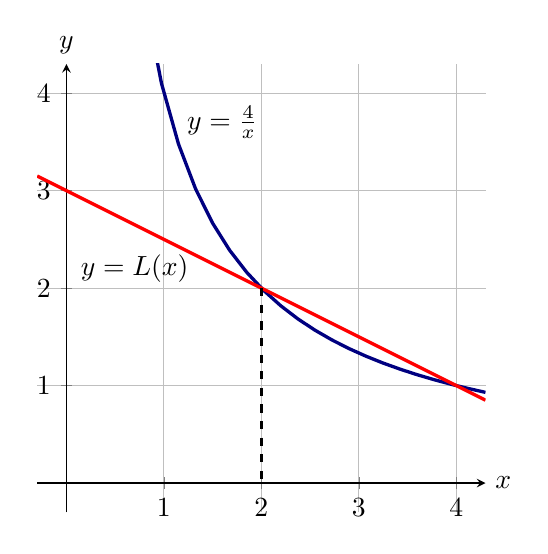
\begin{tikzpicture}
    \begin{axis}[
        xmin=-0.3,xmax=4.3,ymin=-0.3,ymax=4.3,
        clip=true,
        unit vector ratio*=1 1 1,
        axis lines=center,
        grid = major,
        ytick={-6,-5,...,4},
 	    xtick={-6,-5,...,6},
        xlabel=$x$, ylabel=$y$,
        every axis y label/.style={at=(current axis.above origin),anchor=south},
        every axis x label/.style={at=(current axis.right of origin),anchor=west},
      ]
      \addplot[very thick,penColor,domain=0.1:4.3] plot{4/x};
      \addplot[very thick,red,domain=-0.3:4.3] plot{-(x-2)/2+2};
      \draw[very thick,dashed] (axis cs:2,2) -- (axis cs:2,0);
      
      \node at (axis cs:1.6,3.7) [black] {$y=\frac{4}{x}$};
      \node at (axis cs:0.7,2.2) [black] {$y=L(x)$};
      \end{axis}`
  \end{tikzpicture}
\end{image}

The linear approximation to $f$ at $a=2$ is
\[
L(x) = \answer{4-x}.
\]

Using that linear approximation, we can estimate the value of $\frac{4}{2.8}$ to be about
\[
\frac{4}{2.8} \approx \answer{4-2.8}.
\]

This approximation is an \wordChoice{\choice{overestimate}\choice[correct]{underestimate}} because $f(x)$ is concave \wordChoice{\choice[correct]{up}\choice{down}} and the graph of $L$ lies \wordChoice{\choice{above}\choice[correct]{below}} the graph of $f$ near $a=2$.

The percent error in an approximation is given by
\[
100\frac{|approximation - exact|}{|exact|},
\]
where the exact value is given by a calculator.  In this case our percent error (to the nearest percentage point) in approximating $\frac{4}{2.8}$ is
\[
\textnormal{percent error} = \answer{16}\%.
\]

When $x$ changes from $a=2$ to $a+\Delta x = 2.8$, the change in $y$ is 
\[
\Delta y = f\left(\answer{2.8}\right) - f\left(\answer{2}\right) = \answer{-\frac{4}{7}}.
\]
Now in this case the \textbf{approximate} change in $y$ is
\[
\d{y} = f'\left(\answer{2}\right)\d{x} = \answer{-0.8}.
\]

The picture below shows the graph of $f$ along with the linear approximation to $f$ at $a=2$.  On this diagram are quantities labeled $A$, $B$, $C$, $D$, and $E$.  Correctly identify them below.

\begin{image}
  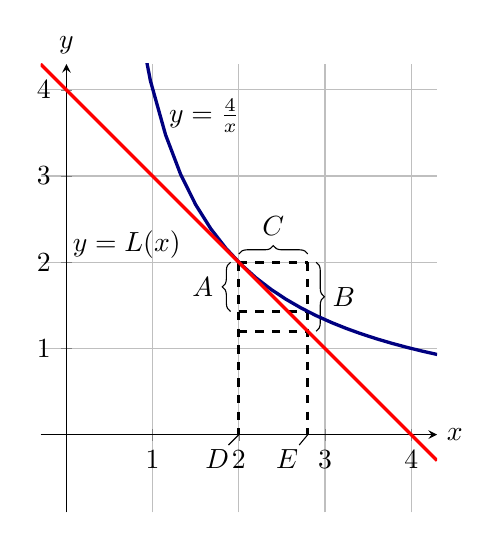
\begin{tikzpicture}
    \begin{axis}[
        xmin=-0.3,xmax=4.3,ymin=-.9,ymax=4.3,
        clip=true,
        unit vector ratio*=1 1 1,
        axis lines=center,
        grid = major,
        ytick={-6,-5,...,4},
 	    xtick={-6,-5,...,6},
        xlabel=$x$, ylabel=$y$,
        every axis y label/.style={at=(current axis.above origin),anchor=south},
        every axis x label/.style={at=(current axis.right of origin),anchor=west},
      ]
      \draw[very thick,dashed] (axis cs:2,2) -- (axis cs:2,0);
      \draw[very thick,dashed] (axis cs:2.8,2) -- (axis cs:2.8,0);
      \draw[very thick,dashed] (axis cs:2,1.2) -- (axis cs:2.8,1.2);
      \draw[very thick,dashed] (axis cs:2,10/7) -- (axis cs:2.8,10/7);
      \draw[very thick,dashed] (axis cs:2,2) -- (axis cs:2.8,2);

	  \draw[decorate,decoration={brace,amplitude=3pt,mirror},xshift=-3pt] (axis cs:2,2) -- (axis cs:2,10/7) node[midway,xshift=-10pt]{$A$};
	  \draw[decorate,decoration={brace,amplitude=3pt},xshift=3pt] (axis cs:2.8,2) -- (axis cs:2.8,1.2) node[midway,xshift=10pt]{$B$};
	  \draw[decorate,decoration={brace,amplitude=3pt},yshift=3pt] (axis cs:2,2) -- (axis cs:2.8,2) node[midway,yshift=10pt]{$C$};
	  \node at (axis cs:2,0) [below left,yshift=-2pt] {$D$};
	  \node at (axis cs:2.8,0) [below left,yshift=-2pt] {$E$};
	  \draw (axis cs:2.8,0) -- (axis cs: 2.7,-0.12);
	  \draw (axis cs:2,0) -- (axis cs:1.88,-0.12);
	        
      \addplot[very thick,penColor,domain=0.1:4.3] plot{4/x};
      \addplot[very thick,red,domain=-0.3:4.3] plot{-(x-2)+2};
      
      \node at (axis cs:1.6,3.7) [black] {$y=\frac{4}{x}$};
      \node at (axis cs:0.7,2.2) [black] {$y=L(x)$};
      \end{axis}`
  \end{tikzpicture}
\end{image}

Chose the correct expression for $A$
\begin{multipleChoice}
\choice{$\d{x}$}
\choice{$\d{y}$}
\choice[correct]{$\Delta y$}
\choice{$a$}
\choice{$a+\Delta x$}
\end{multipleChoice}

Chose the correct expression for $B$
\begin{multipleChoice}
\choice{$\d{x}$}
\choice[correct]{$\d{y}$}
\choice{$\Delta y$}
\choice{$a$}
\choice{$a+\Delta x$}
\end{multipleChoice}

Chose the correct expression for $C$
\begin{multipleChoice}
\choice[correct]{$\d{x}$}
\choice{$\d{y}$}
\choice{$\Delta y$}
\choice{$a$}
\choice{$a+\Delta x$}
\end{multipleChoice}

Chose the correct expression for $D$
\begin{multipleChoice}
\choice{$\d{x}$}
\choice{$\d{y}$}
\choice{$\Delta y$}
\choice[correct]{$a$}
\choice{$a+\Delta x$}
\end{multipleChoice}

Chose the correct expression for $E$
\begin{multipleChoice}
\choice{$\d{x}$}
\choice{$\d{y}$}
\choice{$\Delta y$}
\choice{$a$}
\choice[correct]{$a+\Delta x$}
\end{multipleChoice}

\end{exercise}
\end{document}